% The parts of the Stage 2 report owned by Daniel Perdomo (plan DP-13): cover, section 2, section 4,
% section 5 (Search and deployment) and the Search part of section 7. Section numbers follow the
% list of assignment section 7.1, where the cover is number 1.
%
% Build from docs/report/:  pdflatex search_part.tex && pdflatex search_part.tex
% To assemble the final report, \input the files of sections/ in the main document.
% \pending{...} marks what still depends on the measures: it must not reach the final PDF.
\documentclass[11pt,a4paper]{article}

\usepackage[utf8]{inputenc}
\usepackage[T1]{fontenc}
\usepackage{lmodern}
\usepackage{microtype}
\usepackage[margin=2.4cm,headheight=14pt]{geometry}
\usepackage{graphicx}
\usepackage{booktabs}
\usepackage{tabularx}
\usepackage{array}
\usepackage{enumitem}
\usepackage{float}
\usepackage{xcolor}
\usepackage{listings}
\usepackage{fancyhdr}
\usepackage{titlesec}
\usepackage[hidelinks]{hyperref}

\definecolor{accent}{HTML}{2a78d6}
\definecolor{ink}{HTML}{0b0b0b}
\definecolor{muted}{HTML}{52514e}
\definecolor{codebg}{HTML}{f6f6f4}
\definecolor{rule}{HTML}{d8d7d2}
\definecolor{pendingink}{HTML}{b3261e}

\hypersetup{colorlinks=true,linkcolor=accent,urlcolor=accent,citecolor=accent}

\titleformat{\section}{\Large\bfseries\color{ink}}{\thesection.}{0.6em}{}
\titleformat{\subsection}{\large\bfseries\color{ink}}{\thesubsection}{0.6em}{}
\titlespacing*{\section}{0pt}{1.6em}{0.7em}
\titlespacing*{\subsection}{0pt}{1.2em}{0.5em}

\pagestyle{fancy}
\fancyhf{}
\fancyhead[L]{\small\color{muted}Stage 2 $\cdot$ Service-oriented architecture}
\fancyhead[R]{\small\color{muted}Big Data $\cdot$ ULPGC}
\fancyfoot[C]{\small\thepage}
\renewcommand{\headrulewidth}{0.4pt}

\setlist{itemsep=2pt,topsep=4pt}
\setlength{\parskip}{0.45em}
\setlength{\parindent}{0pt}
\setlength{\emergencystretch}{3em}
\renewcommand{\arraystretch}{1.25}

\lstset{language={}, basicstyle=\ttfamily\footnotesize, backgroundcolor=\color{codebg}, frame=single,
  rulecolor=\color{rule}, framesep=4pt, xleftmargin=6pt, xrightmargin=6pt, breaklines=true,
  columns=fullflexible, keepspaces=true, showstringspaces=false, aboveskip=8pt, belowskip=8pt}

\newcolumntype{L}[1]{>{\raggedright\arraybackslash}p{#1}}
\newcommand{\code}[1]{\texttt{#1}}
\newcommand{\pending}[1]{\par\medskip{\color{pendingink}\textbf{[PENDING]} #1}\par\medskip}

\begin{document}

\begin{titlepage}
\thispagestyle{empty}
\vspace*{2.5cm}
{\color{accent}\rule{\linewidth}{1.2pt}}\\[0.8cm]
{\Huge\bfseries Search Engine Project\par}
\vspace{0.4cm}
{\LARGE Stage 2: Service-Oriented Architecture\par}
\vspace{0.6cm}
{\color{accent}\rule{\linewidth}{1.2pt}}
\vspace{2cm}

\begin{tabular}{@{}>{\bfseries}L{3.4cm}L{10.5cm}@{}}
Course & Big Data $\cdot$ Grado en Ciencia e Ingeniería de Datos $\cdot$ Universidad de Las Palmas de Gran Canaria \\
Academic year & 2026/2027 \\
Group name & BigData-Ulpgc \\
Members & Daniel Rodríguez Alonso --- 79072763M \\
 & Daniel Perdomo Medina --- 54173402F \\
 & Carlos Falcón Brito --- 54149163X \\
Repository & \url{https://github.com/BigData-Ulpgc/stage_2} \\
\end{tabular}
\vfill
\end{titlepage}

\tableofcontents
\clearpage

\setcounter{section}{1}
\section{Introduction and objectives}
\label{sec:intro}

Stage 1 built and measured the data layer of a search engine over the books of Project Gutenberg: a
datalake, an inverted index and a metadata store. Stage 2 turns that data layer into a system of
cooperating services that keeps working while books are being added and users are searching, all on a
single machine.

The system has four kinds of process. \textbf{Ingestion} downloads books and stores them in the datalake.
\textbf{Indexing} adds complete books to the index and publishes new versions of it. \textbf{Search}
answers the front-end. The \textbf{Control Module} decides what has to be done and when, without doing
any of the work itself. They coordinate through Hazelcast and share their results through the datalake and
MongoDB. A front-end only sees one public API, behind nginx.

The objectives of the stage, and how the system meets them, are:

\begin{itemize}
  \item \textbf{Clear contracts.} Every HTTP endpoint is specified in OpenAPI and classified as
        front-end, internal or operational, and the interactions that are not HTTP have their own
        contracts (Section~\ref{sec:api}).
  \item \textbf{Correct behaviour under concurrency.} A book is only indexed once complete, each book
        is processed by one worker at a time, and a search never sees a partially published version.
  \item \textbf{Survival of failures.} A worker that dies loses its lease and its book returns to the
        queue. If Hazelcast loses its state, the Control rebuilds it from what is persistent. If a Search
        replica dies, nginx sends the request to another one.
  \item \textbf{Reproducible deployment.} One command starts every process with fixed resource limits,
        and the number of replicas and threads of each service is configurable
        (Section~\ref{sec:deployment}).
  \item \textbf{Evidence.} The APIs are checked automatically against the running system, and the
        benchmarks identify what limits performance on one machine, keeping client concurrency, threads
        and replicas apart (Section~\ref{sec:benchmarks}).
\end{itemize}

Everything runs on one host by design: replicas and threads share its CPU, memory and disk. What these
measures say about one machine does not establish how the system will scale on the Stage 3 cluster.


\setcounter{section}{3}
\section{API design and contracts}
\label{sec:api}

The full specifications are in the repository, one OpenAPI document per service because every service has
a \code{GET /status}: \code{api/openapi.yaml} (Search), \code{api/indexing-openapi.yaml},
\code{api/ingestion-openapi.yaml} and \code{api/control-openapi.yaml}. The inventory of every endpoint is
\code{api/endpoints.md}. This section summarises them.

\subsection{Front-end use cases}

A front-end needs three things, and it reaches them only through nginx on port 8080:

\begin{itemize}
  \item Search books by keywords, optionally by author, language and year, one page at a time.
  \item Show the details of one book.
  \item Offer the available filters: the languages and the range of years of the published index.
\end{itemize}

\begin{table}[H]
\centering\small
\begin{tabularx}{\linewidth}{@{}L{4.6cm}L{1.6cm}X@{}}
\toprule
\textbf{Endpoint} & \textbf{Provider} & \textbf{Purpose} \\
\midrule
\code{GET /search} & Search & Keyword search (AND) with filters and pagination \\
\code{GET /books/\{book\_id\}} & Search & Metadata of one published book \\
\code{GET /search/filters} & Search & Languages and year range of the published index \\
\bottomrule
\end{tabularx}
\caption{Front-end inventory. All are read-only, so they are safe to retry.}
\end{table}

\subsection{Internal and operational interfaces}

These are consumed by another service or by an operator, never by the front-end. Only the Control Module
is published on the host, on \code{127.0.0.1}; the others are reached by name inside the Docker network.

\begin{table}[H]
\centering\small
\begin{tabularx}{\linewidth}{@{}L{4.9cm}L{2.4cm}X@{}}
\toprule
\textbf{Endpoint} & \textbf{Consumer} & \textbf{Completion} \\
\midrule
\code{POST /ingest/\{book\_id\}} & operators, validation & Done: the book is stored, or was already available \\
\code{GET /ingest/status/\{book\_id\}} & operators, validation & Done (read-only) \\
\code{GET /ingest/list} & operators, validation & Done (read-only) \\
\code{POST /index/update/\{book\_id\}} & operators, validation & Done: indexed, but not visible until published \\
\code{POST /index/publish} & Control Module & Done: \code{CURRENT} points to the returned version \\
\code{POST /index/rebuild} & operators & Accepted: continues in the background \\
\code{GET /index/status} & Control, operators & Done (read-only) \\
\code{POST /control/jobs} & operators, benchmarks & Accepted (202): follow it with \code{/control/status} \\
\code{GET /control/status} & operators, benchmarks & Done (read-only) \\
\code{GET /control/tasks/\{book\_id\}} & operators, validation & Done (read-only) \\
\code{POST /control/retry-failed} & operators & Accepted: the books are back in their queue \\
\midrule
\code{GET /status} (every service) & Docker healthcheck, operators & Done. Liveness only: it does not depend on MongoDB or Hazelcast \\
\bottomrule
\end{tabularx}
\caption{Internal inventory, and the operational endpoint in the last row.}
\end{table}

\subsection{Parameters, pagination and errors}

\code{GET /search} requires \code{q}, tokenised with the same \code{Tokenizer} as Indexing, so a query made
only of stopwords has no terms and is rejected. \code{author} matches part of the name, ignoring case;
\code{language} is an ISO 639-1 code; and \code{year} has four digits. Filters combine with AND.

Pagination uses \code{offset} (default 0) and \code{limit} (default 20, at most 100). \code{total} counts every
match, not only the page, and a valid search without matches answers 200 with an empty list. Results are
ordered by ascending \code{book\_id}, behind a \code{ResultRanking} interface that lets the order change
without touching the search. A ranking by relevance would also need term frequencies, which the index does
not store.

Every response of Search carries \code{index\_version}, the one version it was computed from. All services
share one error format:

\begin{lstlisting}
{"error": {"code": "INVALID_PARAMETER", "message": "limit must be ...", "field": "limit"}}
\end{lstlisting}

\begin{table}[H]
\centering\small
\begin{tabularx}{\linewidth}{@{}L{1.2cm}L{5.4cm}X@{}}
\toprule
\textbf{Status} & \textbf{Code} & \textbf{Meaning} \\
\midrule
400 & \code{MISSING\_PARAMETER}, \code{INVALID\_PARAMETER} & The request is wrong; \code{field} says where \\
404 & \code{NOT\_FOUND} & Unknown book, or a route that does not exist \\
503 & \code{INDEX\_NOT\_READY} & Nothing has been published yet \\
503 & \code{STORAGE\_UNAVAILABLE} & MongoDB does not answer; retry later \\
503 & \code{COORDINATION\_UNAVAILABLE} & The Control has no connection to Hazelcast \\
500 & \code{INTERNAL\_ERROR} & Our bug: the details go to the log, not to the client \\
\bottomrule
\end{tabularx}
\caption{Main errors. Each specification lists those of its service.}
\end{table}

\subsection{Contracts that are not HTTP}

Most of the work between services does not use HTTP:

\begin{itemize}
  \item \textbf{Coordination} (\code{api/contracts/coordination.md}): the Hazelcast map \code{book-state},
        the queues \code{ingest-queue} and \code{index-queue}, the topic \code{index-events} with the
        \code{IndexPublished} event, the lock of the index writer, leases and the transitions of a book.
  \item \textbf{Datalake readiness} (\code{api/contracts/datalake-readiness.md}): ranges of folders and the
        \code{<id>.\_READY} marker, written last, which says a book is complete.
  \item \textbf{Publication in MongoDB:} \code{index\_books}, \code{index\_meta} (\code{CURRENT}) and
        \code{index\_publications}. Switching \code{CURRENT} changes one document, so a new version appears
        all at once. The index itself is not copied, because the entries of a written book never change.
\end{itemize}

\pending{Link the contract of the publication when \code{api/contracts/index-publication.md} exists (plan,
owner Daniel Rodríguez). Today the inventory cites the plan, which is not in the repository.}

\subsection{Validation evidence}

The APIs can be checked without a front-end at three levels, all with their expected results:

\begin{itemize}
  \item \code{scripts/validate-api.sh}: every check with one command against the running system, ending
        with exit code 1 if any fails. On the 15 books of the sample dataset it gives 64 correct, 0 failed and
        0 skipped, both with the books loaded directly and with the same books processed by the complete
        flow (Control, Ingestion, Indexing and publication).
  \item \code{StackValidationTest}: the same contract in JUnit, also checking the shape of the JSON.
  \item \code{http/*.http}: examples to run by hand, documented in \code{http/README.md}.
\end{itemize}

They cover keyword search, each filter alone and combined, valid searches without results, invalid parameters,
pagination, the internal endpoints, and the read-only mounts of the datalake. A check only reports
\textit{skipped} for an endpoint that answers 501; a route that disappears is a failure. The expected answers
were compared with the original texts, so they are not a copy of what the API returns. The load tests refuse
to measure if this validation fails.

\section{Microservice implementation: Search and deployment}
\label{sec:search}

\subsection{Search Service}

Search is written in Java 17 with Javalin and Gson, and implements \code{api/openapi.yaml}. It never writes and
mounts no volume: everything it needs is in MongoDB, which makes it easy to move to another machine in Stage 3.
Its main classes are:

\begin{table}[H]
\centering\small
\begin{tabularx}{\linewidth}{@{}L{4.3cm}X@{}}
\toprule
\textbf{Class} & \textbf{Responsibility} \\
\midrule
\code{SearchApi} & Validates the parameters and writes the HTTP answers \\
\code{SearchEngine} & Runs one query on one snapshot \\
\code{IndexSnapshotLoader} & Builds a snapshot of the published version from MongoDB \\
\code{IndexSnapshot} & Immutable: version, published ids and their metadata \\
\code{SnapshotHolder} & Keeps the current snapshot in an \code{AtomicReference} \\
\code{SnapshotRefresher} & Checks \code{CURRENT} periodically and on demand, on one thread \\
\code{PublicationEvents} & Listens to \code{IndexPublished} in the background \\
\code{MongoPostingSource} & Reads the posting lists of the terms with one query \\
\bottomrule
\end{tabularx}
\caption{Structure of the Search Service.}
\end{table}

\textbf{One query.} \code{SearchEngine} reads the posting lists of the terms. It walks the shortest list and
keeps an id only if every other list has it, using binary search, so the cost depends on the rarest term. Then
it drops the ids that the snapshot does not publish, applies the filters on the metadata in memory, orders all
the matches and cuts the requested page.

\textbf{Consistency.} Indexing may already have written books that are not published, so Search must not show
everything it finds. Each request takes the snapshot once when it starts and works only with that one, so it
cannot mix versions, and it reports that version as \code{index\_version}. The loader reads \code{CURRENT} first
and then the books up to that version. A book keeps the version in which it first became visible, so whatever
moment the loader runs, it sees all of a version and never part of the next one. Replacing the snapshot is one
atomic write: no request waits for it, and no thread can see one half built.

\textbf{Reloading.} A new version reaches Search in two ways. The \code{IndexPublished} event makes it react at
once, but it is only a wake-up: its content is not used, and whoever receives it reads \code{CURRENT} from
MongoDB. The check of \code{CURRENT} every \code{SEARCH\_POLL\_SECONDS} (5 s) is the backup for lost events.
Both run the reload on the same thread, so a slow reload never blocks the Hazelcast thread and two
reloads never overlap. If a reload fails, the replica keeps serving the snapshot it has.

A failure found in testing shows why both are needed. The ringbuffer of a new Hazelcast cluster starts again at
sequence 0, while the subscription keeps waiting at the sequence it had reached. After restarting both members,
Search received no event until as many versions had been published, and only the periodic check kept it up to
date. Each reconnection now subscribes again and checks \code{CURRENT} once; a test restarts the cluster
repeatedly and publishes one event at a time, as Indexing does.

\textbf{Availability.} Search starts even if MongoDB or Hazelcast are down, or nothing has been published.
\code{/status} answers from the first moment, because connecting to Hazelcast happens in the background after the
HTTP server starts. Searches answer 503 until a version is loaded. If Hazelcast is down, Search keeps working with
the periodic check; if MongoDB is down, searches answer 503 \code{STORAGE\_UNAVAILABLE} and recover by themselves.

\textbf{Concurrency.} A request runs on a thread of the Jetty pool, whose maximum is explicit in
\code{SEARCH\_HTTP\_THREADS}: 250, the default value of Javalin 6.1.3, with a minimum of 8 and a 60~s idle
timeout. These threads share only immutable data, so they need no lock. One \code{MongoClient} per process has a pool
of \code{SEARCH\_MONGO\_POOL\_SIZE} connections (50), and a request that waits more than 5~s for one answers
503 instead of keeping its thread busy for the 2 minutes of the driver's default.

\textbf{Browsers.} \code{CORS\_ORIGINS} lists the origins allowed to call the API from a web page; an invalid value
stops the start.

\subsection{Deployment}
\label{sec:deployment}

\code{docker compose up} starts everything on one host from \code{docker-compose.yml} and \code{.env}, which
holds every default. All Java services use one multi-stage template, \code{docker/service.Dockerfile}, with the
Maven module as an argument.

\begin{table}[H]
\centering\small
\begin{tabularx}{\linewidth}{@{}L{2.5cm}L{1.3cm}L{3.1cm}L{1.9cm}X@{}}
\toprule
\textbf{Service} & \textbf{Replicas} & \textbf{Published on the host} & \textbf{Datalake} & \textbf{Limits} \\
\midrule
\code{nginx} & 1 & 8080 & none & 0.5 CPU, 128 MiB \\
\code{search} & 1--4 & none & none & 2 CPU, 1 GiB each \\
\code{indexing} & 1 & none & read-only & 2 CPU, 1 GiB \\
\code{ingestion} & 1--4 & none & read-write & 1 CPU, 512 MiB each \\
\code{control} & 1 & 7000, local only & read-only & 0.5 CPU, 384 MiB \\
\code{hz-1}, \code{hz-2} & 2 & 5701, 5702, local only & none & 1 CPU, 768 MiB each \\
\code{mongo} & 1 & 27017, local only & none & 2 CPU, 1 GiB \\
\bottomrule
\end{tabularx}
\caption{Containers of the deployment. One replica of each adds up to about 5.7~GB of memory limits.}
\end{table}

\begin{itemize}
  \item \textbf{Replicas.} \code{docker compose up -d --scale search=3} is enough: nginx
        (\code{scripts/nginx.conf}) does round-robin over the replicas, which it finds with the DNS of Docker and
        looks up again while running.
  \item \textbf{Failures.} The public API is read-only, so nginx can safely repeat a request on another replica if
        one dies. It does not do so on a 503: a replica that answers is alive, and the others would answer the same.
        Killing one of 3 replicas during a test lost none of 2,000 requests.
  \item \textbf{Permissions.} Only Ingestion can write in the datalake, and Docker enforces it. Hazelcast has no
        authentication, so only nginx listens on all the interfaces.
  \item \textbf{Fixed resources.} Every container has limits, and the heap is a fixed share of its memory, so the
        benchmarks can be repeated and report what they used.
  \item \textbf{Monitoring.} \code{scripts/monitor.sh} records the CPU and memory of each container and the load of
        the host as CSV. A sample of the containers takes about 2~s, because of \code{docker stats}.
\end{itemize}

\textbf{Replicas and threads are different things.} A thread shares its process with the others, including the
snapshot. A replica is another process with its own memory, its own snapshot and its own connection pool, reached
through nginx. Both share the CPU, memory and disk of the host, and all the replicas share one MongoDB.


\setcounter{section}{6}
\section{Benchmarks and results: Search}
\label{sec:benchmarks}

This part covers Search; Section~7 of the final report consolidates it with the other services. The scripts and
the instructions to repeat every measure are in \code{benchmarks/search/}.

\subsection{Reference machine}

All the valid measures come from one machine, idle during the run. \code{host.txt} records each run.

\begin{table}[H]
\centering\small
\begin{tabularx}{\linewidth}{@{}L{3.2cm}X@{}}
\toprule
CPU & Intel Core i7-9750H, 2.60 GHz: 6 cores, 12 logical CPUs \\
Memory and storage & 16 GB, NVMe SSD \\
Operating system & Ubuntu 24.04, Linux 7.0 \\
JVM & OpenJDK 21.0.12, heap fixed at 4 GB for JMH \\
Power & Plugged in, balanced energy profile \\
Code & commit \code{263fb9f} for JMH \\
\bottomrule
\end{tabularx}
\caption{Reference machine of the benchmarks.}
\end{table}

\textbf{A deviation in the JMH run.} A loop of \code{docker stats} left over from an earlier test was running during the
measures. It takes little CPU, and the errors of the results are small, but the machine was not completely idle, as
\S6.3 of the assignment asks.

\pending{Add the Docker version and the commit of the load tests from their \code{host.txt}. If JMH is measured
again without that process, replace the numbers of this section and remove the paragraph above.}

\subsection{Microbenchmarks with JMH}

The JMH classes are in \code{search-service/src/test/java/.../benchmark}, so they are not part of the service jar,
and they run directly on the host. They measure \code{SearchEngine} on a synthetic index held in memory, without
MongoDB or HTTP, with 200, 10,000 and 100,000 books. Each configuration runs 5 warm-up and 10 measurement iterations
of 1~s in 2 separate JVMs with a fixed heap of 4~GB, and each scenario compares its result with an independent
calculation before measuring.

\begin{table}[H]
\centering\small
\begin{tabularx}{\linewidth}{@{}L{3.6cm}X@{}}
\toprule
\textbf{Benchmark} & \textbf{What changes} \\
\midrule
Intersection & Number of books and of terms in the query \\
Filters & Number of books and which filter \\
Pagination & Number of books, position of the page (0, 50 and 99 \%) and its size (20 and 100) \\
Threads & 1, 2, 4 and 8 threads on the same intersection, with 100,000 books \\
\bottomrule
\end{tabularx}
\caption{JMH experiments.}
\end{table}

\textbf{Limitation.} Each term is assigned to books at random and independently, while real words tend to appear
together. These results compare the cost of each step; they do not predict the response time of real queries.

In the synthetic index, \code{common} is in 50~\% of the books, \code{frequent} in 30~\%, \code{medium} in 10~\%
and \code{rare} in 1~\%, so the number of matches of each query is known in advance. Every value below is the
mean time of one search, with its 99.9~\% error in the CSV files.

\begin{table}[H]
\centering\small
\begin{tabularx}{\linewidth}{@{}Xrrrr@{}}
\toprule
\textbf{Query} & \textbf{Matches} & \textbf{200 books} & \textbf{10,000} & \textbf{100,000} \\
\midrule
\code{common} & 50 \% & 2.7 µs & 362 µs & 6.06 ms \\
\code{common frequent} & 15 \% & 1.5 µs & 288 µs & 3.45 ms \\
\code{common frequent medium} & 1.5 \% & 0.8 µs & 78 µs & 0.85 ms \\
\code{common rare} & 0.5 \% & 0.3 µs & 4.3 µs & 0.15 ms \\
\bottomrule
\end{tabularx}
\caption{JMH: intersection without filters, first page of 20, one thread.}
\end{table}

\begin{figure}[H]
\centering
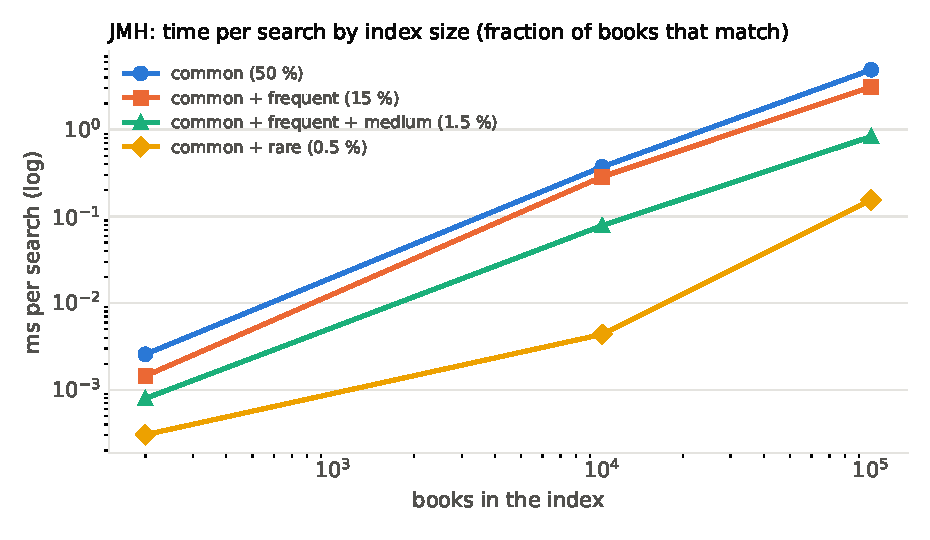
\includegraphics[width=0.82\linewidth]{figures/jmh_intersection.pdf}
\caption{Time per search against the size of the index, both axes logarithmic.}
\end{figure}

\textbf{What the intersection shows.}
\begin{itemize}
  \item \textbf{The cost follows the number of matches, not only the length of the lists.} With 100,000 books the
        four queries all read the list of \code{common}, 50,000 ids, yet they range from 6.06~ms to 0.15~ms. A rarer
        term makes the shortest list shorter, so the intersection walks fewer ids, and fewer matches are then checked
        against the snapshot, filtered and sorted.
  \item \textbf{Ten times more books cost more than ten times as much at the top of the scale.} From 10,000 to
        100,000 books, \code{common} goes from 362~µs to 6.06~ms, 16.7 times. Sorting every match grows faster than
        linearly, and the larger lists no longer fit in the CPU caches. These are our explanations; they were not
        measured separately.
\end{itemize}

\textbf{Filters.} With 100,000 books and the query \code{common}, no filter takes 4.97~ms. The language filter adds
5~\% and the author filter 12~\%, because it compares strings ignoring case; all of them together, 14~\%. The year
filter takes 8~\% less, because it leaves fewer books to sort. Filters run in memory on the metadata of the snapshot,
after the intersection, so they never add a query to MongoDB.

\textbf{Pagination.} The position of the page does not change the cost: with 100,000 books, the first page, the middle
one and one near the end all take about 4.84--4.87~ms, within the error, and so do pages of 100 results. Every search
does all the work (intersection, filters, ordering of every match) before cutting the page, and the cut itself costs
almost nothing. The other side is that the first page is not cheaper either: a user who only looks at 20 results
pays for all of them. Caching the result of a query until the next version is published would avoid it, because a
snapshot never changes.

\begin{figure}[H]
\centering
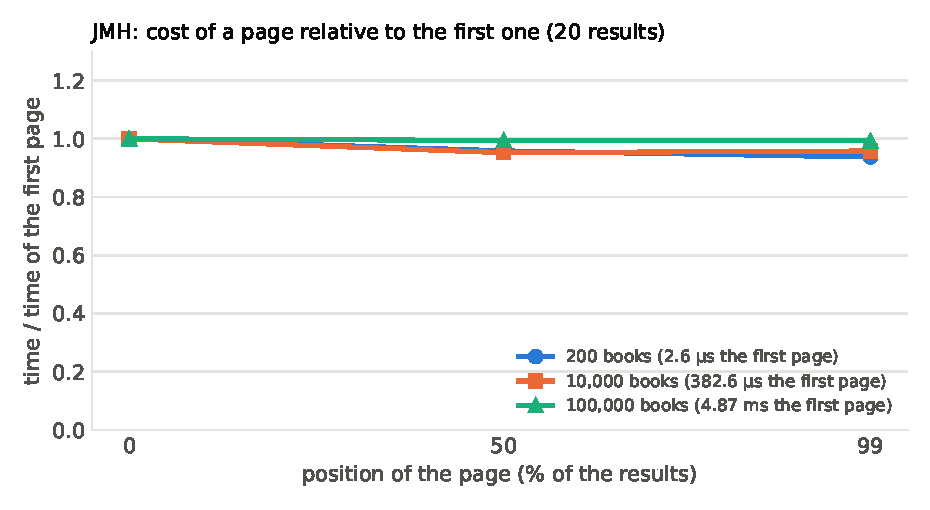
\includegraphics[width=0.82\linewidth]{figures/jmh_pagination.pdf}
\caption{Time of a page relative to the first page, pages of 20 results.}
\end{figure}

\textbf{Threads.} \code{SearchEngine} has no state of its own and the snapshot is immutable, so several threads
search at once without locks. With 100,000 books and \code{common frequent}, 2 threads complete 1.9 times as many
searches per second as one, 4 threads 3.6 times and 8 threads 5.7 times. Each search becomes slower as threads are
added, from 3.31~ms with one to 4.62~ms with eight. The threads do not wait for each other, but they share the CPU
caches and the memory bandwidth, and 8 threads exceed the 6 physical cores of the machine.

\begin{figure}[H]
\centering
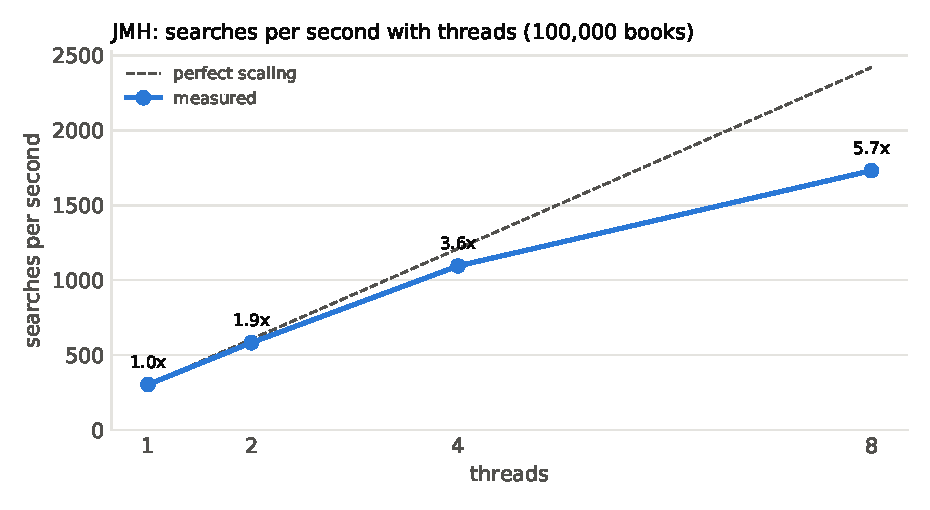
\includegraphics[width=0.82\linewidth]{figures/jmh_threads.pdf}
\caption{Searches per second with 1 to 8 threads, against perfect scaling.}
\end{figure}

This is the cost of the code alone. A real search adds MongoDB, which returns the posting lists, HTTP and nginx: the
load tests measure them.

\subsection{Load tests}

\code{LoadGenerator} sends \code{GET /search} through nginx with \code{shared/queries.txt}, and checks each answer
against the total and version it obtained first: more replicas must not change the results. Before measuring, the
script runs \code{validate-api.sh}. Each configuration is repeated 3 times with 15~s of warm-up and 30~s of measure,
and one factor changes at a time:

\begin{table}[H]
\centering\small
\begin{tabularx}{\linewidth}{@{}L{1.9cm}L{5.2cm}X@{}}
\toprule
\textbf{Experiment} & \textbf{What changes} & \textbf{Fixed} \\
\midrule
Clients & 1, 8, 32, 128, 256 clients with 1, 2 and 4 replicas & 250 threads, pool of 50, nginx with 2 CPUs \\
Threads & 16 and 64 Jetty threads, with the same clients & 1 replica, pool of 50, nginx with 2 CPUs \\
Pool & 10 and 100 MongoDB connections, with 32, 128 and 256 clients & 1 replica, 250 threads, nginx with 2 CPUs \\
nginx & 0.5 CPUs, the limit of the deployment, with 32, 128 and 256 clients & 1 replica, 250 threads, pool of 50 \\
Index size & 200 real books, and 100,000 synthetic ones if available & Same as the clients experiment \\
\bottomrule
\end{tabularx}
\caption{Load experiments. Client concurrency, threads per process and replicas are kept apart.}
\end{table}

\textbf{Why nginx has 2 CPUs here.} Short trial runs showed that nginx, with the 0.5 CPUs of the deployment,
saturated before Search and hid the effect of everything else. The experiments therefore give it 2 CPUs and measure
the 0.5 limit separately.

\textbf{Limitations.}
\begin{itemize}
  \item The generator runs on the same machine as the system, so it competes with it for CPU.
  \item It is a closed loop: under saturation, clients wait instead of queuing more requests, so latencies are lower
        than with requests arriving at a fixed rate.
  \item With 4 replicas the limits of the containers add up to 14 CPUs, which may exceed the host. Then the limits no
        longer bound each container, and the replicas compete for the same cores.
\end{itemize}

\pending{Insert the tables and figures of \code{results/analysis/}: throughput and p95 against clients for each number
of replicas, the effect of threads and of the pool, and CPU and memory per container.}

\subsection{Analysis}

\pending{Write it from the measures, without assuming the outcome. It must answer: at how many clients does the
throughput stop growing, and what happens to p95 and p99? Which container reaches its CPU limit first (Search, MongoDB
or nginx)? Do replicas and threads help, and if not, why? Is the pool of 50 connections too small or too large, as this
was an estimate? Does a larger index move the bottleneck to MongoDB? Were there errors or wrong results?}

\pending{State what was not measured and why: full pipeline under load, 100,000 books if DR-16 did not arrive.}


\end{document}
